\section{Results}
Our simulator was designed to be similar to the experiments made by Sugiyama
et al.\cite{sugiyama} for simple data comparison. Figure \ref{normal_postime}
shows the absolute position on the circular road of 60 cars with
normal drivers for $ 150 \unit{s} $. In this plot it can be seen that several
of the cars came to a complete stop after $ 30 \unit{s} $. These stops can
then be characterized as waves \cite{mit} moving backwards in the
lane with a constant speed of $ 13 \unit{km/h} $.\\\\

\begin{figure}[H]
    \begin{center}
    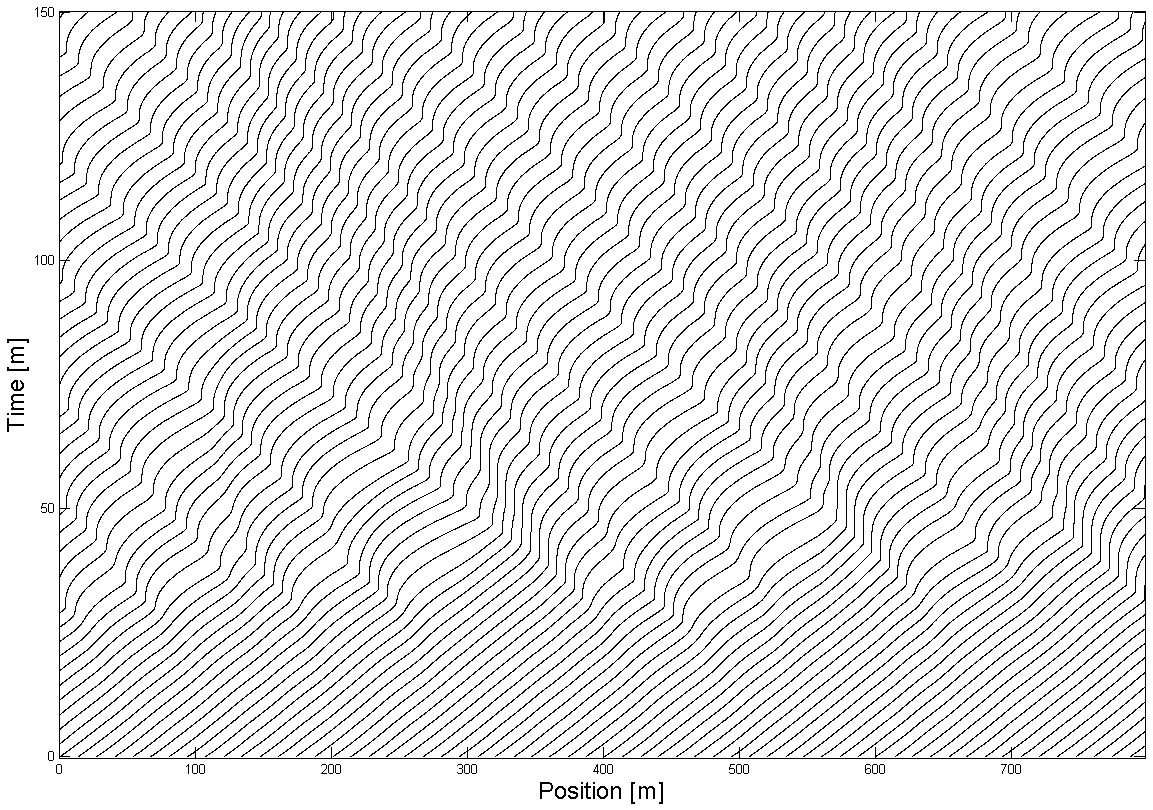
\includegraphics[width=1.0\textwidth]{normal_60cars_50kmh.png}
    \caption{\label{normal_postime}
Absolute position of 60 cars for $ 150 \unit{s} $. Data from simulator. After
$ 30 \unit{s} $ phantom jams were emerging.}
    \end{center}
\end{figure}

Simular plots for cars equipped with ACC and EACC can be seen in
Appendix \ref{app_postime_plot}. In these cases the cars were never forced to
stop completely. When the cars were equipped with ACC the jams did not occur
until after $ 300 \unit{s} $. If they instead were equipped with the enhanced
model the jams did not occur until after $ 1200 \unit{s} $. In both these
cases the waves were travelling backwards at a speed of $ 15 \unit{km/h} $.\\\\

\begin{figure}[h!]
    \begin{center}
    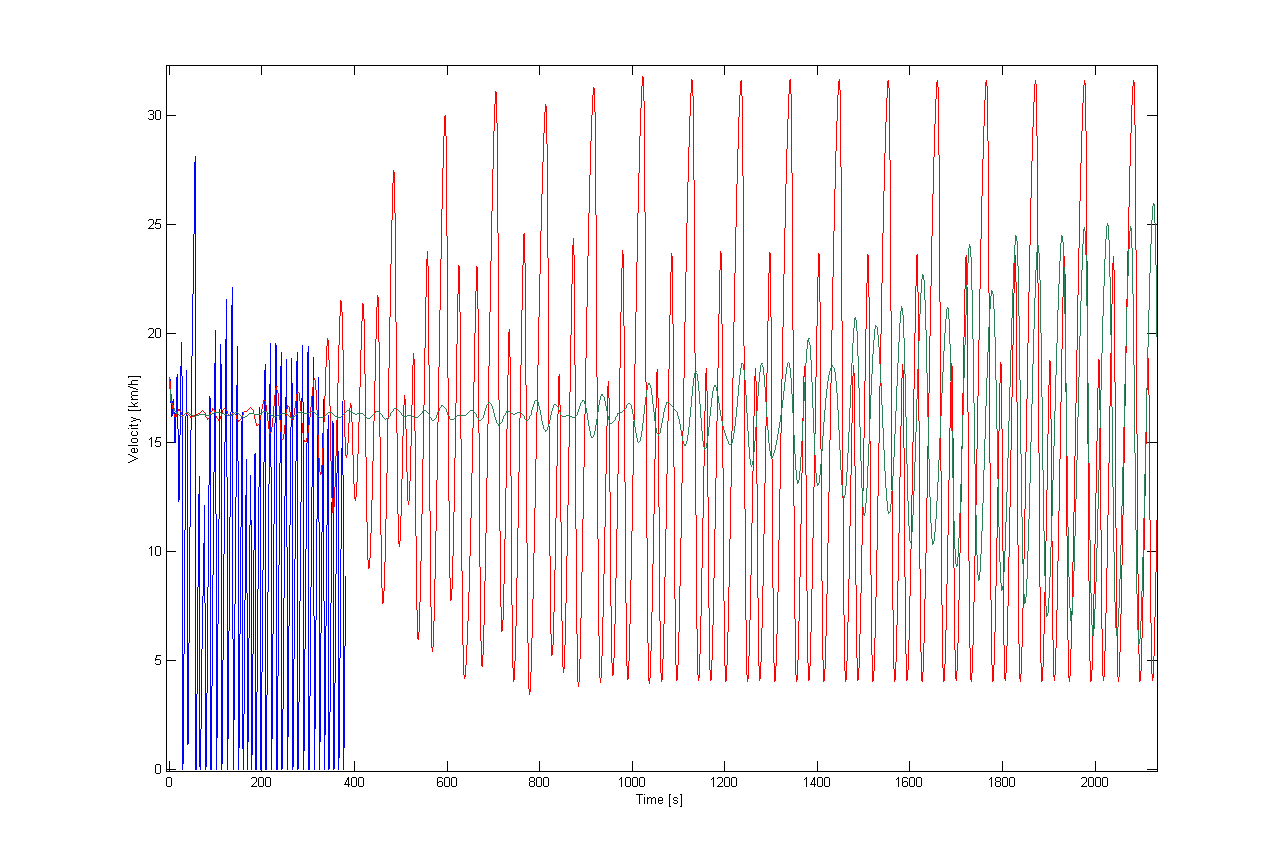
\includegraphics[width=1.0\textwidth]{velocity.png}
    \caption{\label{velocity}Velocity of one specific car on the road during
2000 seconds using the three different models. Blue curve - normal driver. Red
curve ACC. Green curve - EACC.}
    \end{center}
\end{figure}

The differences between the systems is clearly illustrated by data in figure
\ref{velocity}. In the model with a normal driver instability occured almost
immediately and on many occasions the car was forced to a complete stop. When
the ACC-system was implemented there were still large oscillations but
they occured later and the average velocity was higher than for the normal
driver. The enhanced model was able to to keep the traffic stable for about $
800 \unit{s} $ and then oscillations occured, but with lower amplitude.

\subsection{Comparison of Performance}
We measured performance of the different systems as average traffic flow
$ [\unit{vehicles/h}] $ as a function of average traffic density
$ [\unit{vehicles/km}] $. The speed limit was fixed to $ 50 \unit{km/h} $ in all
experiments. Data is presented in fig \ref{performance}.\\\\

\begin{figure}[h!]
    \begin{center}
    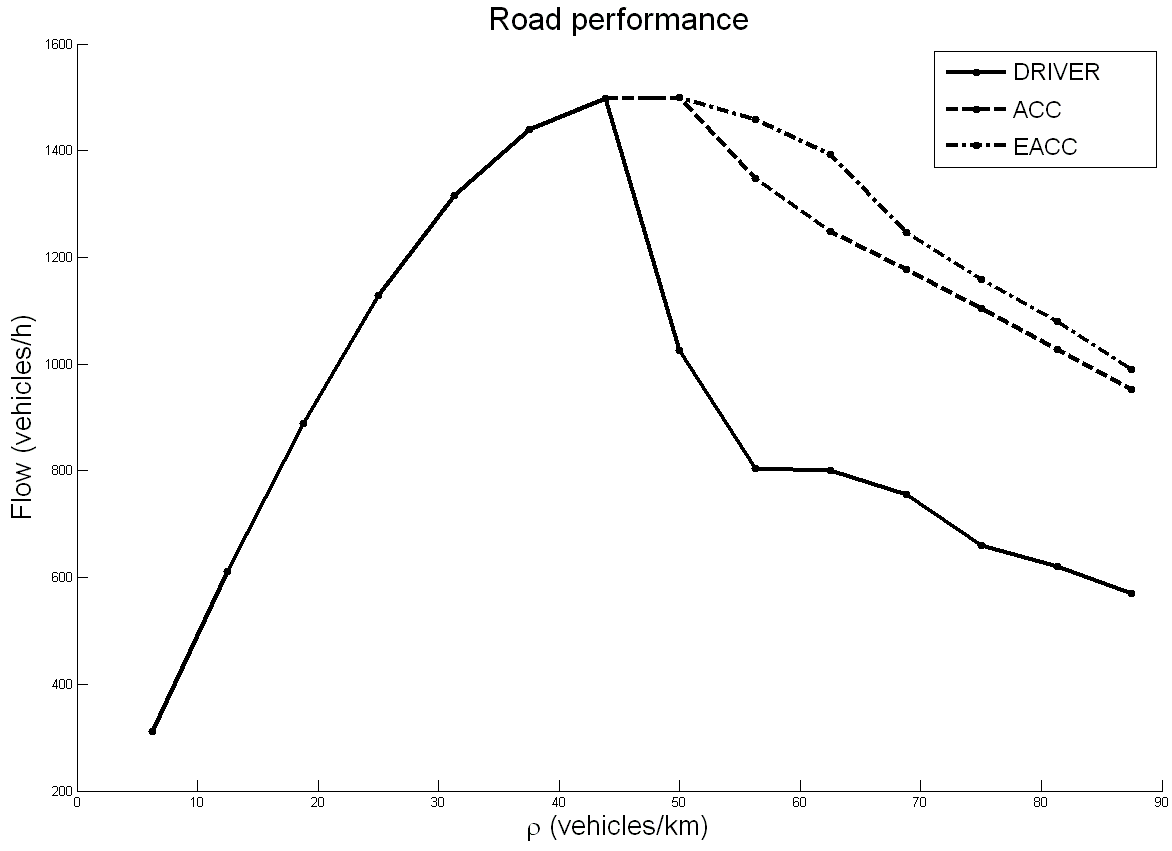
\includegraphics[width=1.0\textwidth]{flowdensity_2.png}
    \caption{\label{performance}
Traffic flow as a function of traffic density. Data from simulator.
$SpeedLimit=50 \unit{km/h}$. Traffic flow was measured when traffic conditions had stabilized.}
    \end{center}
\end{figure}

Initially, the performance of all three systems grow linearly as traffic
was light enough to allow all cars to keep maximum allowed speed. As traffic
grew denser, the cars had to slow down to keep constant time headway. All
three systems follow the same performance curve until a density of $ 50.0
\unit{vehicles/km} $ is reached. At this point, phantom jams appeared in the
normal driver system and traffic flow droped dramatically. For the Adaptive
Cruise Control system and the Enhanced Adaptive Cruise Control system,
phantom jams were first observed at $ 56.3 \unit{vehicles/km} $ and $ 68.8
\unit{vehicles/km} $ respectively. Figure \ref{performance} also shows that
the performance of these two systems was not reduced by the phantom jams as
severely as for the normal driver system.



